% This is a LaTeX thesis template for Monash University.
% to be used with Rmarkdown
% This template was produced by Rob Hyndman
% Version: 6 September 2016

\documentclass{monashthesis}

%%%%%%%%%%%%%%%%%%%%%%%%%%%%%%%%%%%%%%%%%%%%%%%%%%%%%%%%%%%%%%%
% Add any LaTeX packages and other preamble here if required
%%%%%%%%%%%%%%%%%%%%%%%%%%%%%%%%%%%%%%%%%%%%%%%%%%%%%%%%%%%%%%%
\usepackage{epigraph}
\usepackage{multirow}
\usepackage{tabularx}
\usepackage{booktabs}
\usepackage{makecell}
\usepackage{amsmath}


% \epigraphsize{\small}% Default
\setlength\epigraphwidth{8cm}
\setlength\epigraphrule{0pt}

\usepackage{etoolbox}

\makeatletter
\patchcmd{\epigraph}{\@epitext{#1}}{\itshape\@epitext{#1}}{}{}
\makeatother



\author{Thiyanga Shamini Talagala}
\title{Computationally Efficient Forecasting Methods for Large-Scale Real-Time Applications}
\degrees{M.Sc., University of Moratuwa, Sri Lanka \break B.Sc. (Hons), University of Sri Jayewardenepura, Sri Lanka}
\def\degreetitle{Doctor of Philosophy}
% Add subject and keywords below
\hypersetup{
     %pdfsubject={The Subject},
     %pdfkeywords={Some Keywords},
     pdfauthor={Thiyanga Shamini Talagala},
     pdftitle={Computationally Efficient Forecasting Methods for Large-Scale Real-Time Applications},
     pdfproducer={Bookdown with LaTeX}
}


\bibliography{thesisrefs}

\begin{document}

\pagenumbering{roman}

\titlepage

{\setstretch{1.2}\sf\tighttoc\doublespacing}

\hypertarget{copyright-notice}{%
\chapter*{Copyright notice}\label{copyright-notice}}
\addcontentsline{toc}{chapter}{Copyright notice}

© Thiyanga Shamini Talagala (2019).

I certify that I have made all reasonable efforts to secure copyright permissions for third-party content included in this thesis and have not knowingly added copyright content to my work without the owner's permission.

\hypertarget{abstract}{%
\chapter*{Abstract}\label{abstract}}
\addcontentsline{toc}{chapter}{Abstract}

Forecasting is a key activity for any business to operate efficiently. The dramatic increase in the availability of large collections of time series raises the need for developing reliable efficient and automatic algorithms for forecasting. This thesis presents three such algorithms for large-scale applications based on the meta-learning approach. The key idea behind the methodology is the use of a vector of features on each time series, measuring global characteristics of the series. The process starts with an offline phase: train a meta-learner to relate the features of time series to the performance of different forecast models using a large historical collection of time series. The online phase of generating forecasts involves only the calculation of a simple vector of features for any newly given time series and the application of a pre-trained meta-learner to produce the required forecasts.

The first algorithm is FFORMS: Feature-based FORecast Model Selection. FFORMS builds a mapping that relates the features of time series to the `best' forecast model using a random forest. The process of generating forecasts involves the application of the best model for each series. This is a very fast and reliable approach. The FFORMS algorithm is evaluated using the time series from the M1, M3 and M4 competitions and is shown to yield accurate forecasts comparable to several benchmarks and other commonly used automatic approaches for time series forecasting. Furthermore, model-agnostic machine learning interpretability tools are used to explore what is happening under the hood of the FFORMS algorithm. In particular, the thesis explores \emph{which} features are the most important for the choice of model selection; \emph{where} they are most important, that is, for the overall classification process or, within specific class of models or a set of multiple classes of models; \emph{how} these features link with the predicted outcome; and \emph{when} and \emph{how strongly} features interact with other features. The results provide valuable insights into how different features and their interactions affect model selection.

The second algorithm, FFORMA (Feature-based FORecast Model Averaging) obtains weights for forecast combinations. The extreme gradient boost algorithm with a custom objective function is used to train a meta-model. The probabilities of each model being best are used as weights for computing a combination forecast. The FFORMA approach achieved second place in the recent M4 forecasting competition \autocite{makridakis2018m4}.

The third algorithm is FFORMPP (Feature-based FORecast Model Performance Prediction). The efficient Bayesian multivariate surface regression approach is used to model forecast error as a function of features calculated from the time series. FFORMPP allows rankings of models according to their relative forecast performance without calculating forecasts from all available models in the pool. Further, a feature-based time series simulation approach is used to obtain a diverse collection of time series to train the meta-learner. In addition, the thesis attempts to visualise the relationships discovered by the meta-learning algorithm. The visualisation approach involves mapping each time series as a point in a two-dimensional instance space, given by the features. This helps to gain insights into why certain models perform better on certain types of time series.

\hypertarget{publications-during-enrolment}{%
\chapter*{Publications during enrolment}\label{publications-during-enrolment}}
\addcontentsline{toc}{chapter}{Publications during enrolment}

This thesis by publication is built around four articles which are at different stages of publication.

\begin{enumerate}
\def\labelenumi{\arabic{enumi}.}
\item
  Chapter \ref{ch:paper2} has been submitted to the \emph{International Journal of Forecasting} for possible publication.

  Talagala, T. S., Hyndman, Rob. J., \& Athanasopoulos, G. (2018). Meta-learning how to forecast time series. Working Paper 6/18. Department of Econometrics \& Business Statistics, Monash University.
\item
  Chapter \ref{ch:paper3} is ready for submission to \emph{Computational Statistics \& Data Analysis}.

  Talagala, T. S., Hyndman, R. J., \& Athanasopoulos, G. (2019). Peeking inside FFORMS: Feature-based forecast model selection. Computational Statistics \& Data Analysis {[}ready for submission{]}.
\item
  Chapter \ref{ch:paper4} has been accepted for publication in the \emph{International Journal of Forecasting} and is currently in press.

  Montero-Manso, P., Athanasopoulos, G., Hyndman, R. J., Talagala, T. S. (2019) FFORMA: Feature-based forecast model averaging. International Journal of Forecasting {[}to appear{]}
\item
  Chapter \ref{ch:paper5} has been submitted to the \emph{International Journal of Forecasting} for possible publication.

  Talagala, T. S., Feng, L., \& Kang, Y. (2019). FFORMPP: Feature-based forecast model performance prediction. International Journal of Forecasting {[}under review{]}.
\end{enumerate}

The contributions in Chapters \ref{ch:paper2} - \ref{ch:paper5} of this thesis were presented at the following events:

\begin{itemize}
\tightlist
\item
  37th International Symposium on Forecasting 2017, Cairns, Australia.
\item
  Young Statisticians Conference 2017, Tweed Heads, NSW, Australia. \newline A Statistical Society of Australia travel award grant was received to attend the conference.
\item
  Young Stats Showcase hosted by the Statistical Society of Australia, Victorian Branch, Australia, in September 2017.
\item
  38th International Symposium on Forecasting 2018, Boulder, Colorado, USA, in June 2018 \newline
  An International Institute of Forecasters travel award grant was received to attend the conference.
\item
  2018 Joint Statistical Meetings (JSM2018), Vancouver, British Columbia, Canada, in August 2018
\item
  useR! 2018, Brisbane, Australia, in July 2018
\item
  Invited talk, Central University of Finance and Economics, Beijing, China, in March 2019
\item
  39th International Symposium on Forecasting, Thessaloniki, Greece, in June 2019 \newline An International Institute of Forecasters travel award grant was received to attend the conference.
\item
  useR! 2019, Toulouse, France, in July 2019
\end{itemize}

\hypertarget{declaration}{%
\chapter*{Declaration}\label{declaration}}
\addcontentsline{toc}{chapter}{Declaration}

I hereby declare that this thesis contains no material which has been accepted for the award of any other degree or diploma at any university or equivalent institution and that, to the best of my knowledge and belief, this thesis contains no material previously published or written by another person, except where due reference is made in the text of the thesis.

This thesis includes one original paper published in a peer reviewed journal and three submitted publications. The core theme of the thesis is feature-based large-scale time series forecasting. The ideas, development and writing up of all the papers (with the exception of Chapter \ref{ch:paper4}) in the thesis were the principal responsibility of myself, the student, working within the Department of Econometrics and Business Statistics, Monash University, under the supervision of Professor Rob J Hyndman and Professor George Athanasopoulos.

The inclusion of co-authors reflects the fact that the work came from active collaboration between researchers and acknowledges input into team-based research.

In the case of Chapter 2-5 my contribution to the work involved the following:

\begin{table}
\centering\footnotesize\tabcolsep=0.12cm
\begin{tabular}{|p{1cm}|p{2cm}|p{1.5cm}|p{3.5cm}|p{3.5cm}|p{1.5cm}|}
\hline
\rowcolor[gray]{.1}  \textbf{\color{white}Thesis Chapter}  & \textbf{\color{white}Publication Title}  & \textbf{\color{white}Status (published, in press, accepted or returned for revision)}  &  \textbf{\color{white}Nature and} \color{white}{\%} \textbf{\color{white}of student contribution} & \textbf{\color{white}Co-author name(s) Nature and} \color{white}{\%} \textbf{\color{white}of Co-author’s contribution} &  \textbf{\color{white}Co-author(s), Monash student Y/N} \\ \hline
2 & Meta-learning how to forecast time series  & returned for revision  & Formulating the approach, construction of research design, implementation, data analysis and interpretation, software development, writing the first draft (80\%)   & 1) Rob J Hyndman, input into manuscript (10\%) \newline 2) George Athanasopoulos, input into manuscript (10\%)  & \multicolumn{1}{c|}{N}   \\
\hline
3 & Peeking inside FFORMS: Feature-based forecast model selection  & ready for submission  & Formulating the approach, construction of research design, implementation, data analysis and interpretation, software development, writing the first draft (90\%)   & 1) Rob J Hyndman, input into manuscript (5\%) \newline 2) George Athanasopoulos, input into manuscript (5\%)  & \multicolumn{1}{c|}{N}   \\
\hline
4 & FFORMA: Feature-based forecast model averaging & published  & Formulating the approach, construction of research design, initiate writing the first draft (6\%)   & 1) Pablo Montero-Manso, input into manuscript (80\%) \newline 2) George Athanasopoulos, input into manuscript (7\%) \newline 3) Rob J Hyndman, input into manuscript (7\%)   & \multicolumn{1}{c|}{N}    \\
\hline
5 & FFORMPP: Feature-based forecast model performance prediction & submitted  & Formulating the approach, construction of research design, implementation, data analysis and interpretation, software development, writing the first draft (80\%)   & 1) Feng Li, input into manuscript (10\%)  \newline 2) Yanfei Kang, input into manuscript (10\%)   & \multicolumn{1}{c|}{N}   \\
\hline
\end{tabular}
\end{table}

\newpage

I have not renumbered sections of submitted or published papers in order to generate a consistent presentation within the thesis.

\textbf{Student name:} Thiyanga Shamini Talagala
\vspace{-0.15cm}

\textbf{Student signature:}
\includegraphics[width=0.15\textwidth]{img0000.png} \hspace{5cm}\textbf{Date:} 22 August 2019

\hypertarget{acknowledgements}{%
\chapter*{Acknowledgements}\label{acknowledgements}}
\addcontentsline{toc}{chapter}{Acknowledgements}

UseR 2019! in Toulouse, France, is where I gave my last talk as a PhD student. The conference gala dinner was held at the Cite' de l'espace, Toulouse. At Cite' de l'espace, I had an opportunity to experience what it feels like to be inside a true space shuttle and learn how they operate. A space shuttle needs a massive amount of energy to fight against gravitational pull, but once it has launched, the space shuttle just glides along easily. What matters for the space shuttle is the first push off the ground. Two powerful side rockets help a shuttle to leave the gravitational pull.

I am extremely thankful to my supervisors, Professor Rob J Hyndman and Professor George Athanasopoulos, for being two powerful side rockets. I thank them for giving me that first push in the right direction and for making sure I saw this project to its completion. I would like to thank them for their endless energy and guidance.

I would like to thank the PhD directors, Professor Gael Martin and Professor Farshid Vahid, for their valuable support and encouragement. I am thankful to Professor Di Cook, Dr Souhaib Ben Taieb and Dr Klaus Ackerman, the members of my PhD panel, for their constructive suggestions and helpful feedback. I am also very grateful to Professor Scott Sisson for his encouraging advice.

Chapter \ref{ch:paper5} of this thesis is a research collaboration with Associate Professor Feng Li of Central University of Finance and Economics in China and Associate Professor Yanfei Kang of Beihang University, China. I am grateful to both of them for inviting me to visit China to work on the project presented in Chapter \ref{ch:paper5}. Further, I would like to thank the members of their forecasting team for their wonderful hospitality. I am grateful to Central University of Finance and Economics, Beijing, China, for providing financial support during the visit. Further, the work presented in Chapter \ref{ch:paper4} is a research collaboration with Dr Pablo Montero-Menso. I am thankful to him for several hours of discussion on the subject.

I am very grateful to Monash University for awarding me the Monash Graduate Scholarship, and to the Faculty of Business and Economics for offering me the Faculty Postgraduate Research Scholarship. Further, I gratefully acknowledge the research funding provided by the Australian Research Council Centre of Excellence for Mathematical and Statistical Frontiers. I was also awarded two travel awards from the International Institute of Forecasters to attend the 38th International Symposium on Forecasting in Boulder, USA, and the 39th International Symposium on Forecasting in Thessaloniki, Greece. This support is gratefully acknowledged.

The computational resources and services used in this thesis were supported in part by the Monash eResearch Centre and eSolutions Research Support Services through the use of the MonARCH (Monash Advanced Research Computing Hybrid) HPC cluster. Special thanks to Philip Chen and Simon Michnowicz from the Monash E-research Centre for their time spent answering my questions and help provided in using the parallel supercomputing facility. To the members of the NUMBAT research group, the MONASH data fluency group and R-Ladies Melbourne, many thanks for making the environment a stimulating, enjoyable and supporting place for research.

I would also like to thank Elite Editing for copyediting the thesis. The editorial intervention by Elite Editing was restricted to Standards D and E of the Australian Standards for Editing Practice. I wish to extend a special thanks to the Monash Graduate Research team for their support along the way. I would also like to express my appreciation to the administrative staff of the Department of Econometrics and Business Statistics, especially Clare Livesey for her friendly support and assistance throughout!

This journey would not have been possible without the support of my family. I am extremely lucky to have done my PhD together with my sister, Priyanga Dilini Talagala. Getting full scholarships from Australia's prestigious Monash University to do our PhDs is another big accomplishment we achieved together. I thank my father and mother for their endless encouragement and invaluable inspiration. This thesis is dedicated to my family, father, mother and sister, who have all shown me great love and continuous support in many ways all these years.

\clearpage\pagenumbering{arabic}\setcounter{page}{0}

\hypertarget{ch:intro}{%
\chapter{Introduction}\label{ch:intro}}

\epigraph{Essentially, all models are wrong, but some are useful.}{--- \textup{George E. P. Box}, 1987}

The words of famous British statistician George Box encapsulate the essence of model selection. This statement is particularly valid for forecast model selection. For many decades, researchers have been developing increasingly sophisticated
models for forecasting. From a theoretical and computational point of view, these models are elegant and efficient algorithms, which makes them appealing candidates for many applications. However, given the large number of models, it is challenging to identify which one is likely to generate the most accurate forecasts for a given time series. Even though various models for time series forecasting have been developed, little research has contributed to advice on when each model is beneficial. Moreover, as stated by \textcite{georgoff1986manager}, the main issue facing forecasters is not the need for new or more sophisticated models, but the need to derive better approaches for forecast model selection. Since a trial-and-error approach is an extremely time consuming search process, researchers need to identify more efficient search strategies. The aim of this thesis is to develop new frameworks that will help in forecasting large numbers of time series completely automatically.

\hypertarget{background-of-the-study}{%
\section{Background of the study}\label{background-of-the-study}}

The advent of modern technologies has enabled businesses and companies to collect ever more data. Of these, time series data are everywhere and play a key role in business decision-making processes. For example, large-scale businesses, such as Facebook \autocite{taylor2018forecasting} and Walmart \autocite{seaman2018considerations}, need to forecast many millions of time series for capacity planning to optimise resource allocation, set targets to evaluate performance relative to baseline, and so on. Hence, accurate forecasts for these series are immensely valuable. The brute force solution is simply to try out all the candidate models on the problem at hand and select the model that performs best over the test period. This model is then used to forecast future values of the time series. However, this approach is not feasible in practice, especially when there are tens or hundreds of millions of series to forecast. The alternative solution is `aggregate selection', in which a single method is used to compute forecasts for all time series \autocite{fildes1989evaluation}. According to the no-free-lunch concept, there is no single model that performs best on all kinds of time series \autocite{wolpert1997no}. Since neither solution is ideal, there is a need for a more general and flexible framework to assist in forecasting large numbers of time series.

In an attempt to answer the question `Which forecast model performs best on a given series?', Spyros Makridakis organised the Makridakis Competitions, also known as M-Competitions. The M-Competitions have had a profound influence on the field of time series forecasting \autocite{hyndman2019brief}. The findings of these competitions also point to many important
research directions and conclusions \autocite{makridakis2001response}. Of these, two are particularly important for the problem addressed by this thesis. First, the characteristics of time series are useful for identifying suitable models for forecasting \autocites{armstrong2001s}{tashman2001m3}. Second, forecasters should be able to explain the conditions under which each method works best \autocites{hyndman2001s}{makridakis2001response}. To this end, this thesis investigates the utility of the characteristics of time series referred to as \emph{features} in addressing the problem of large-scale time series forecasting. Feature-based analysis of time series has several advantages over raw point analysis: it facilitates data visualisation and understanding; it acts as a dimension-reduction tool, thereby reducing storage requirements and computational time; it handles time series with unequal lengths \autocite{guyon2003introduction}; among others.

A few researchers have explored the benefit of using time series features to select suitable forecasting methods. \textcite{collopy1992rule} introduced 99 rules based on 18 features of time series to make forecasts for economic and demographic time series. \textcite{meade2000evidence} uses 25 features of time series to predict the relative performance of nine different models. \textcite{petropoulos2014horses} examine the effect of seven time series features (seasonality, trend, cycle, randomness, length, inter-demand interval and coefficient of variation) on predicting the performance of 14 popular models through regression analysis. The authors argue for a `horses for courses' approach to discovering the extent to which the features of time series are useful in predicting the model performance. In an attempt to answer the question raised by \textcite{hyndman2001s} in the M3 competition discussion `why some methods work well and others do not' \textcite{kang2017visualising} try to visualise the algorithm performance in the instance space defined by six features. A more detailed description of the literature is given in Chapter \ref{ch:paper2}.

Although many researchers have highlighted the usefulness of features in forecast model selection, only a few studies have reported success against benchmarks and other commonly used approaches in forecasting. Revisiting this literature reveals significant gaps. Possible reasons for these gaps are i) an inadequate number of features were used; ii) the selected features were not useful for the purpose; iii) possible limitations in the modelling framework used (for example, linear regression models that focus on the global relationship in the data do not incorporate local relationships into the model); and iv) a lack of diversity in the training set of time series used to build the model. In this thesis, the aim is to design feature-based time series forecasting algorithms for large-scale applications and fill in the noticeable gaps in the literature.

\hypertarget{meta-learning}{%
\section{Meta-learning}\label{meta-learning}}

The feature-based forecast algorithms proposed in Chapters \ref{ch:paper2}, \ref{ch:paper4} and \ref{ch:paper5} are based on a meta-learning approach.
A framework for algorithm selection was first proposed in the seminal paper of \textcite{rice1976}. Rice's algorithm selection framework builds a mapping that relates the features of the problem instances with the performance of different algorithms. The machine-learning community use the same idea, calling it `meta-learning'. Although Rice's idea has been around since 1976, not many applications using his idea have been made until recently. However, with the rapid development of information technologies and the emergence of an era of big data, Rice's algorithm selection problem has attracted the attention of many disciplines and provides a promising solution to algorithm selection problems in various domains. \textcite{smith2009cross} provides a comprehensive review of applications of this approach. However, despite its widespread popularity, several researchers have pointed out that it is not entirely clear from Rice's framework how the mapping is done from features to performance of different algorithms. The work was later extended and improved in a few different ways \autocites{smith2012measuring}{kotthoff2016algorithm}. The methodological framework used in this study is shown in Figure \ref{fig:frameworkch1}. The offline and online phases are shown in blue and red respectively. A meta-learner is trained during the offline phase and is then used to select an appropriate model for a new time series in the online phase. The success of a meta-learning framework depends on four main factors: i) problem space, ii) feature space, iii) algorithm space and iv) performance space. These are now described in detail.

\begin{figure}[h]

{\centering 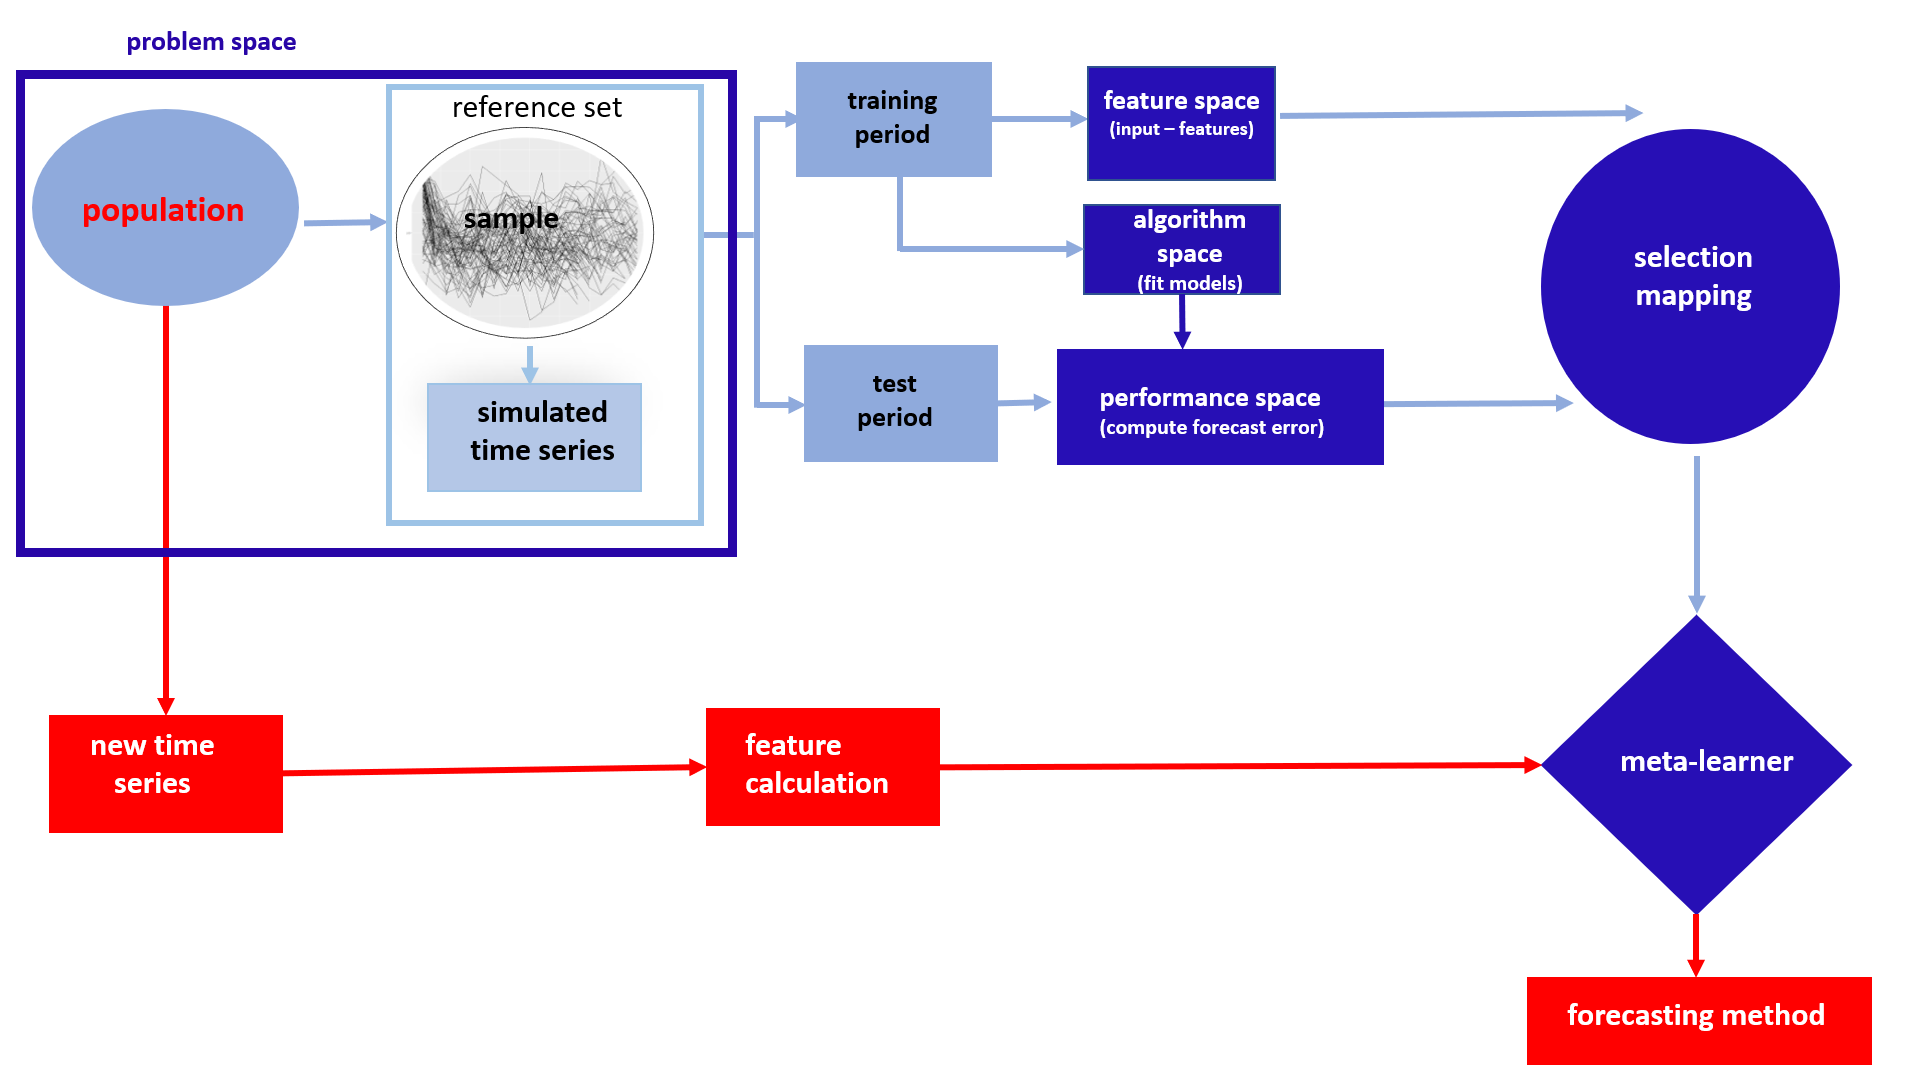
\includegraphics[width=1.05\linewidth,height=0.4\textheight]{chap1metalearning} 

}

\caption{The methodological framework. The offline phase is shown in blue and the online phase in red.}\label{fig:frameworkch1}
\end{figure}

\hypertarget{problem-space}{%
\subsection{Problem space}\label{problem-space}}

The dataset used for the study is called the problem space. In this thesis, the time series of M1, M3 \autocite{makridakis2000m3} and M4 competitions \autocite{makridakis2018m4} form the problem space. \textcolor{black}{The M-competition data were a sample of time series collected from several domains such as demographics, finance, business and economics.} \autoref{mcomp} \textcolor{black}{shows the classification of the M-competition series according to frequency and domain.} A single time series is called \emph{an instance} in the problem space. Prediction accuracy of a meta-learner strongly depends on the instances used to train the meta-learner. In addition to the time series from the M-Competitions, simulated time series are used to increase the diversity of the problem space. The different approaches used to simulate time series are explained in Chapters \ref{ch:paper2}, \ref{ch:paper3} and \ref{ch:paper5}. Further, it is important to note that instances are required that are similar to the time series that are forecasted in the online phase of the algorithm.

\begin{table}[!h]
\centering\scriptsize\tabcolsep=0.12cm
\caption{The composition of M-competition data: the number of time series by domain and frequency category}
\label{mcomp}
{\color{black}\begin{tabular}{l|c|rrrrrr|r|}
\hline
\multirow{2}{*}{Period} & \multicolumn{8}{c|}{Domain} \\ \cline{2-9} 
                  &Competition &Demographic  & Finance  & Industry  & Macro  & Micro & Other &  Total\\ \hline
\multirow{3}{*}{Yearly}& M1 & 30  & -  & 35  & 59 & 57  & - & 181 \\ 
                  & M3  & 245  &  58 &  102 & 83 &146  &  11&645  \\ 
                  & M4 &  1088 &  6519 &  3716 &  3903& 6538 &1236  & 23000 \\ \hline
\multirow{3}{*}{Quarterly}& M1 &  39 &  - & 18  & 104 & 42 &  -&  203\\ 
                 & M3  & 57  &  76 &  83 &  336&  204&  -&  756\\ 
                 & M4 & 1858  & 5305  & 4637  &5315  &  6020& 865 & 24000 \\ \hline
\multirow{3}{*}{Monthly}& M1 &  75 & -  & 183  & 156 & 203 & - &  617\\ 
                 & M3 & 111  & 145  & 334   & 312 & 474 & 52  & 1428 \\  
                 & M4 & 5728  & 10987  & 10017  & 10016 & 10975 & 277 & 48000 \\ \hline
Weekly           & M4 &  24 &  164 &  6 & 41 & 112 & 12 & 359 \\ 
Daily            & M4 & 10  & 1559  &  422 & 127 & 1476 & 638 & 4227 \\ 
Hourly           & M4 &  0 &0   & 0  &  0&  0&  414&  414\\ \hline
\end{tabular}}
\end{table}

\hypertarget{feature-space}{%
\subsection{Feature space}\label{feature-space}}

The feature space is characterised by a set of measurable characteristics of the instances in the problem space. The features can also be considered summary statistics of time series. John W. Tukey was the first to come up with the idea of `features', which he called cognostics: computer aided diagnostics \autocite{tukey1988computer}. A few decades later, his idea was rebranded and used under different names. A broad range of features exists that can be used to summarise time series \autocite{fulcher2014highly}. The choice of features should take account of the final goal of the research question. Further, features of time series play a central role in both online and offline phases of the meta-learning framework. These constraints introduce the need for careful consideration of the feature selection process in the frameworks. The following properties of features are considered:

\begin{enumerate}
\def\labelenumi{\roman{enumi})}
\item
  Informative. Most of the features introduced in the literature aim to identify different patterns in time series. In contrast in this thesis, the interest is in using features to identify the best forecasting model(s) for a given series. Hence, the features considered should provide sufficient distinction between different instances in terms of which is the most suitable model(s) for forecasting.
\item
  Interpretability. The features used should provide meaningful interpretations of the instance characteristics so that practitioners can gain maximum insight into the problem space. Further, this helps explain reasons for the predictions of the meta-learner and gain trust in the proposed frameworks.
\item
  Time and computational cost. Features play a central role in both offline and online phases of the algorithm. To make predictions quickly during the online phase, the features considered should be easy and quick to compute without heavy computational cost.
\item
  Applicability. Features should be computable for a broad range of problem instances, rather than being restricted by different conditions, such as length, non-stationarity and other properties of time series.
\end{enumerate}

Further, apart from a few exceptions (such as length of series, number of times the time series crosses the median and the number of flat spots in the series), most of the features considered here are independent of scale and are ergodic: asymptotically independent of the length of the time series. A more detailed description of the features is given in Chapters \ref{ch:paper2}, \ref{ch:paper3} and \ref{ch:paper4}.

\hypertarget{algorithm-space}{%
\subsection{Algorithm space}\label{algorithm-space}}

A suitable set of candidate models to include in the portfolio forms the algorithm space. In this thesis twelve methods implemented in the \texttt{forecast} package in R \autocite{forecast} are considered for the algorithm space. This is the first time such a large collection of algorithms has been considered in a time series meta-learning framework. The algorithm space includes (The R functions are given in parentheses):

\begin{enumerate}
\def\labelenumi{\roman{enumi})}
\tightlist
\item
  Random walk with drift (\texttt{rwf} with drift=TRUE)
\item
  Random walk model (\texttt{rwf} with drift=FALSE)
\item
  Seasonal naive (\texttt{snaive})
\item
  White noise process
\item
  Theta method (\texttt{thetaf}) -- this method became the winner of the M3 competition \autocite{makridakis2000m3}
\item
  TBATS (\texttt{tbats}) models introduced by \textcite{de2011forecasting}
\item
  Neural network forecasts (\texttt{nnetar})
\item
  automated ARIMA algorithm (\texttt{auto.arima})
\item
  exponential smooting (ETS) algorithm (\texttt{ets})
\item
  STL-AR (\texttt{stlm} with model function \texttt{ar}) -- seasonal and trend decomposition using loess with autoregressive (AR) modelling of the seasonally adjusted series
\item
  MSTL-ETS (\texttt{mstl} with model function \texttt{ets}) -- first, a multiple seasonal decomposition is applied to the time series and then the seasonal naive is used to forecast the seasonal components; then, the automated ETS algorithm is used to forecast the seasonally adjusted series.
\item
  MSTL-ARIMA (\texttt{mstl} with model function \texttt{auto.arima}) -- first, a multiple seasonal decomposition is applied to the time series and then the seasonal naive is used to forecast the seasonal components; then, the automated ARIMA algorithm is used to forecast the seasonally adjusted series.
\end{enumerate}

The methods considered in viii)-xii), involve fully or partially use of the automated ARIMA algorithm of \textcite{Hyndman2008} or the automated ETS algorithm of \textcite{Hyndman2002} to select the appropriate either ARIMA class model or ETS models. Next, the main steps of these algorithms are summarised.

\hypertarget{automated-exponential-smoothing-ets}{%
\subsubsection{\texorpdfstring{Automated exponential smoothing (\texttt{ets})}{Automated exponential smoothing (ets)}}\label{automated-exponential-smoothing-ets}}

Exponential smoothing methods were introduced in the late 1950s \autocites{Brown59}{Brown63}. This framework was later extended by \textcite{gardner1985exponential} and \textcite{Hyndman2002}. Because of their computational simplicity and interpretability, they became widely used in practice. A classification of 15 exponential smoothing methods is presented in \autoref{table1}. Each model can have an additive or multiplicative error, giving 30 different models. Out of these 30 models, only 19 models are numerically stable. Further, multiplicative trend models give poor forecasts, which leaves 15 models.

\begin{table}[!htp]
\centering
\caption{Classification of exponential smoothing methods}
\label{table1}
\begin{tabular}{l|ccc}
\hline
\multirow{2}{*}{Trend component} & \multicolumn{3}{c}{Seasonal Component} \\ \cline{2-4} 
                  &   N (None)    &  A (Additive)     &   M (Multiplicative)    \\ 
 N (None)                 &   N, N    &   N, A    &   N, M    \\ 
 A (Additive)                &   A, N    &   A, A    &  A, M     \\ 
 $A_d$ (Additive damped)                &  A$_d$, N     &   A$_d$, A    &    A$_d$, M   \\ 
  M (Multiplicative)                &   M, N    &    M, A   &    M, M   \\ 
  $M_d$ (Multiplicative damped)                &    M$_d$, N   &  M$_d$, A     & M$_d$, M      \\ \hline
\end{tabular}
\end{table}

The steps involved are summarised below \autocite{Hyndman2008}:

\begin{enumerate}
\def\labelenumi{\arabic{enumi}.}
\item
  For each series, apply each of the 15 models that are appropriate for the data.
\item
  For each model, optimise the parameters (smoothing parameters and initial values for the states) using maximum likelihood estimation.
\item
  Select the best model using the corrected Akaike's Information Criterion (AICc) and produce forecasts using the best selected model.
\end{enumerate}

\hypertarget{automated-arima-modelling-auto.arima}{%
\subsubsection{\texorpdfstring{Automated ARIMA modelling (\texttt{auto.arima})}{Automated ARIMA modelling (auto.arima)}}\label{automated-arima-modelling-auto.arima}}

ARIMA is one of the most popular models for time series forecasting. One of the common difficulties in ARIMA modelling is the order selection process. \textcite{Hyndman2008} developed a framework to automate this process. The steps involved are summarised below:
For non-seasonal data, ARIMA\((p, d, q)\) models are considered and for seasonal data ARIMA\((p, d, q)(P, D, Q)_m\) are considered.

\begin{enumerate}
\def\labelenumi{\arabic{enumi}.}
\item
  Select the number of differences \(d\) and \(D\) via unit root tests.
\item
  Try four possible models to start with:
\end{enumerate}

\begin{enumerate}
\def\labelenumi{\roman{enumi})}
\tightlist
\item
  ARIMA\((2, d, 2)\) if \(m=1\) and ARIMA\((2, d, 2)(1, D, 1)_m\) if \(m > 1\).
\item
  ARIMA\((0, d, 0)\) if \(m=1\) and ARIMA\((0, d, 0)(0, D, 0)_m\) if \(m > 1\).
\item
  ARIMA\((1, d, 0)\) if \(m=1\) and ARIMA\((1, d, 0)(1, D, 0)_m\) if \(m > 1\).
\item
  ARIMA\((0, d, 1)\) if \(m=1\) and ARIMA\((0, d, 1)(0, D, 1)_m\) if \(m > 1\).
\end{enumerate}

\begin{enumerate}
\def\labelenumi{\arabic{enumi}.}
\setcounter{enumi}{2}
\item
  Select the model with the smallest AICc from step 2. This becomes the current model.
\item
  Consider up to 13 variations on the current model:
\end{enumerate}

\begin{enumerate}
\def\labelenumi{\roman{enumi})}
\tightlist
\item
  Vary one of \(p\), \(q\), \(P\) and \(Q\) from the current model by \(\pm\) 1.
\item
  \(p\), \(q\) both vary from the current model by \(\pm\) 1.
\item
  \(P\), \(Q\) both vary from the current model by \(\pm\) 1.
\item
  Include or exclude the constant term from the current model.
  Repeat step 4 until no lower AICc can be found. For more details, please refer to \textcite{Hyndman2008}.
\end{enumerate}

\hypertarget{algorithm-performance-space}{%
\subsection{Algorithm performance space}\label{algorithm-performance-space}}

Algorithm performance space is characterised by a set of metrics used to evaluate the performance of different algorithms on the instances in the problem space. Mean absolute scaled error (MASE) introduced by \textcite{hyndman2006another} is mainly used throughout the thesis for evaluate point forecasts. Let \(y_t\) and \(\hat{y}_t\) denote the observed and forecast values at time \(t\), respectively. Then, MASE is defined by

\[\text{MASE}=\frac{\frac{1}{H}\sum_{h=1}^H |y_{T+h}-\hat{y}_{T+h|T}|}{\frac{1}{n-m}\sum_{t={m+1}}^{T}|y_t - y_{t-m}|}.\]

where \(H\) is the length of the forecast horizon, \(T\) is the length of the training period of the time series and \(m\) is the frequency of the time series. The MASE is independent of the scale of the data. In addition to MASE, symmetric mean absolute percentage error (sMAPE) is used in Chapter \ref{ch:paper3} and Chapter \ref{ch:paper4} because the M4 competition forecasts are evaluated based on both MASE and sMAPE \autocite{M4compguide}. The sMAPE is simply

\[\text{sMAPE}=\frac{1}{H}\sum_{h=1}^H\frac{200|y_h-\hat{y}_h|}{|y_h|+|\hat{y}_h|}.\]

Prediction intervals are also computed. The performance of 95\% prediction intervals are evaluated based on the mean scaled interval score (MSIS) \autocites{gneiting2007strictly}{M4compguide}. The MSIS is defined as

\[\text{MSIS} = \frac{\frac{1}{H}\sum_{h=1}^{H}(U_h-L_h)+40(L_h-y_h)1\{y_h<L_h\}+40(y_h-U_h)1\{y_h>U_h\}}{\frac{1}{n-m}\sum_{t=m+1}^{T}|y_t-y_{t-m}|},\]
where \(L_h\) and \(U_h\) denote the lower and upper bounds of the prediction intervals at time \(h\), and \(1\) is the indicator function (being 1 if \(y_h\) is within the postulated intervals and 0 otherwise).

\hypertarget{linking-feature-space-and-algorithm-performance-space}{%
\section{Linking feature space and algorithm performance space}\label{linking-feature-space-and-algorithm-performance-space}}

Linking feature space and algorithm performance space is a central part of the meta-learning process. Three modelling approaches are used to model the relationships: i) the random forest algorithm, ii) the extreme gradient boosting algorithm and iii) the efficient Bayesian multivariate surface regression approach.

\hypertarget{random-forest-algorithm}{%
\subsection{Random forest algorithm}\label{random-forest-algorithm}}

The methodological framework presented in Chapter \ref{ch:paper2} is based on the random forest algorithm. A random forest \autocite{breiman2001random} is an ensemble learning method that combines a large number of decision trees using a two-step randomization process. This algorithm combines Brieman's idea of \emph{bagging} and \emph{random selection of features at each node} in each tree. The motivation behind the use of random forest classifiers are: i) it can model complex interactions between features; ii) the modelling framework captures linear and non-linear effects of features through the averaging of large number of decision trees; iii) its robustness against over-fitting the training data; iv) it is easy to handle the problem of imbalanced classes; v) it is a fast approach compared to boosting algorithms and vi) it is fairly easy to implement with available software.

\hypertarget{extreme-gradient-boosting-algorithm}{%
\subsection{Extreme gradient boosting algorithm}\label{extreme-gradient-boosting-algorithm}}

The methodological framework presented in Chapter \ref{ch:paper4} is based on the extreme gradient boosting algorithm. The extreme gradient boosting algorithm, also known as XGBoost, is a tree ensemble model for classification and regression introduced by \textcite{chen2016xgboost}. The algorithm involves fitting a sequence of weak learners (in the case of this thesis, decision trees) on reweighted data. The process starts by fitting a shallow decision tree (i.e.~a weak learner) to the whole space of the training data and obtaining predictions. Then, the data are weighted according to the predictions obtained in the previous step (higher weights are assigned to misclassified training instances). The second tree is constructed based on these weighted data. This process is repeated until the stopping criterion is met. The predictions based on all trees are combined through a weighted majority vote (in the case of classification) or weighted sum (in the case of regression) to obtain the final prediction of the model. The concept is similar to the gradient boosting algorithm \autocite{friedman2001greedy} but more efficient. The XGBoost algorithm benefits from a regularised model formalisation to control overfitting. \textcolor{black}{This can be formalised as follows. Let $N$ be the total number of instances (training examples), $f_i$ is a vector of $m$ features for the $i$th data point and $z_i$ is the $i$th observed value of the outcome. Then the training dataset is defined as}

\vspace*{-\baselineskip}

\[D=\{(f_i, z_i): i =1,\dots, N\}, |D|=N, f_i \in \mathbb{R}^m, z_i \in \mathbb{R}.\]

\textcolor{black}{The objective function of the XGBoost algorithm is}

\vspace*{-\baselineskip}

\begin{align}
\mathbb{L}=\sum_{i=1}^{N}l( z_i, \hat{z_i})+\sum_{k=1}^K \Omega(g_{k}).
\end{align}

\textcolor{black}{This contains two parts, the loss function and the regularization term. The first term $l$ is a differential convex loss function that measures the difference between the predicted value $\hat{z}_i$ and the observed value $z_i$, and the second term $\Omega$ is the regularisation term which measures the complexity of the model and $g_k$ corresponds to individual tree. The objective function in Equation  1.3.1 includes functions as parameters and cannot be optimized using traditional optimization methods in Euclidean space. Instead, training of XGBoost algorithm consists of a sequential calculation process and uses $K$ additive functions to obtain the predicted value $\hat{z_i}^{(t)}$.  For each step $t$ the predicted value is}

\vspace*{-\baselineskip}

\begin{align*} 
\hat{z}_i^{(0)} &=  0 \\ 
\hat{z}_i^{(1)} &=  g_1(f_i) =  \hat{z}_i^{(0)}+g_1(f_i)\\ 
\hat{z}_i^{(2)} &=  g_1(f_i)+g_2(f_i) =  \hat{z}_i^{(1)}+g_2(f_i)\\ 
\dots\\
\hat{z}_i^{(t)} &=  \sum_{k=1}^{t}g_k(f_i) =  \hat{z}_i^{(t-1)}+g_t(f_i).
\end{align*}

\textcolor{black}{Substituting the prediction of the $i$-th instance at the $t$-th iteration $\hat{z}_i^{(t)}$ in the objective function }

\vspace*{-\baselineskip}

\begin{align}
\mathbb{L}^{(t)}= \sum_{i=1}^{N} l(z_i, \hat{z}_i^{(t-1)}+g_t(f_i))+\Omega(g_t).
\end{align}

\textcolor{black}{For each iteration, $g_t$ tree needs to be added to minimise the objective function in Equation 1.3.2. The regularization term is}
\vspace*{-\baselineskip}

\[\Omega(g) = \gamma T + \frac{1}{2}\lambda||\omega||^2,\]
\textcolor{black}{where $\omega$ represents the vector scores in the leaves, $T$ is the number of leaves in the tree, $\gamma$ and $\lambda$ are the regularisation parameters.}

In a typical classification problem, the extreme gradient boosting algorithm is trained to minimise a loss function with respect to classification errors. In this thesis, the classification error is not a concern, but minimising the average forecast error is. Hence, a customised loss function is used to include the information on the forecast error rather than the classification error. Extreme gradient boosting algorithm implementation allows easy changes to the objective function. It only requires the output, the gradient and the Hessian of the objective, whereas other methods require reimplementation of the majority part of the code. A detailed description of the methodology is given in Chapter \ref{ch:paper4}.

\hypertarget{efficient-bayesian-multivariate-surface-regression-approach.}{%
\subsection{Efficient Bayesian multivariate surface regression approach.}\label{efficient-bayesian-multivariate-surface-regression-approach.}}

The methodological framework presented in Chapter \ref{ch:paper5} is based on the efficient Bayesian multivariate surface regression introduced by \textcite{li2013efficient}. This approach has a number of advantages: i) \(\textbf{Y}\) is multivariate, which means several responses are predicted simultaneously; ii) the approach allows for interactions between features; iii) the regression splines used here are able to model the non-linear relationship between features and the response variables; and iv) compared with the other spline-based models, this approach allows the knots to move freely in the feature space, and thus a lower number of knots is usually required. A description of this approach is provided in Chapter \ref{ch:paper5}. The estimation and computation details can be found in \textcite{li2013efficient}.

\hypertarget{objectives-and-thesis-outline}{%
\section{Objectives and thesis outline}\label{objectives-and-thesis-outline}}

This is a `thesis by publication', which consists of an introduction and conclusion with published papers in between. The main goal of the thesis is to provide support to practitioners in forecasting large collections of time series, with vectors of features computed from time series. Centralising on this main goal, the objectives and the structure of the thesis can be outlined as follows.

There are many measurable features of time series. For example, one can characterise a time series by the mean value, or by a measure of strength of seasonality, and so on. The challenge is in uncovering features that will help to select suitable models for forecasting. In response to the results of the M3 competition, \textcite{lawrence2001s} wrote:

\begin{quote}
`What is needed now is analysis to determine what are the specific time series characteristics for which each technique is generally best and also what are the time series characteristics for which it does not really matter which technique (or set of techniques) is chosen?'.
\end{quote}

The \textbf{first} objective of this thesis is to identify a suitable set of features that are useful in selecting a good model for forecasting. Chapter \ref{ch:paper2} and Chapter \ref{ch:paper4} introduce a collection of time series features that are useful in selecting models for forecasting.

The \textbf{second} objective is to use a meta-learning approach with a range of features computed from the time series to recommend the way the forecasts are computed. There are many different ways the large-scale time series forecasting problem can be approached based on the meta-learning framework. Hence, this overreaching goal is divided into three constituent aims.

\begin{enumerate}
\def\labelenumi{\arabic{enumi}.}
\item
  The first aim is to develop a meta-learning framework that will help identify the `best' model for a given series. Chapter \ref{ch:paper2} is dedicated to achieving this aim. A random forest classifier is used to identify the `best' model using time series features. The first approach treats the algorithm selection problem as a classification task. This algorithm is called FFORMS (Feature-based FORecast Model Selection). Chapter \ref{ch:paper3} extends this approach in order to handle high frequency data with multiple seasonal components.
\item
  The second aim is to develop a meta-learning framework to obtain weights for forecast combinations. Chapter \ref{ch:paper4} presents the second algorithm, FFORMA (Feature-based FORecast Model Averaging), in which gradient boosting is used to obtain the weights for forecast combinations. This approach achieved second place in the M4 competition \autocite{makridakis2018m4}.
\item
  The third aim is to develop a meta-learning framework that allows the ranking of models according to their relative performance without calculating forecasts from all available individual models in the pool. Chapter \ref{ch:paper5} is dedicated to achieving this aim. The efficient Bayesian multivariate surface regression approach is used to estimate the forecast error for each model, and then using the predicted errors, the models are ranked to identify the `best' individual model or `best subset' of models to compute forecasts.
\end{enumerate}

In the discussion of the M3 competition \textcite{armstrong2001s} raises the point that researchers often fail to describe under which conditions their method performs well and explain the reasons for the expectations. While the literature has concentrated mainly on the use of meta-learning for algorithm selection, not much effort has been put into identifying what is happening inside the framework. The \textbf{third} objective is to explore the relationship between the features of time series and the choice of different models using the meta-learning frameworks introduced in this thesis. Firstly, Chapter \ref{ch:paper3} addresses this third objective. What is happening under the hood of the FFORMS framework is explored, thereby providing an understanding of what features lead to the different choices of forecast models and how different features influence the predicted outcome. This is accomplished using model-agnostic machine-learning interpretability approaches. Secondly, Chapter \ref{ch:paper5} continues addressing this third objective. The instance space defined by features is further explored to understand how certain features of time series influence model selection and also to explain how these different types of instances are located in the feature space.

The \textbf{fourth} objective is to develop a free and open-source R package for the methods introduced in this thesis. The FFORMS algorithm is implemented in the open source R package \texttt{seer}. The FFORMPP algorithm is implemented in the open source R package \texttt{fformpp}.

Chapter \ref{ch:paper6} concludes summarising the findings of the thesis, describing the software implemented and highlighting areas for future research.

\hypertarget{ch:paper2}{%
\chapter{Meta-learning how to forecast time series}\label{ch:paper2}}

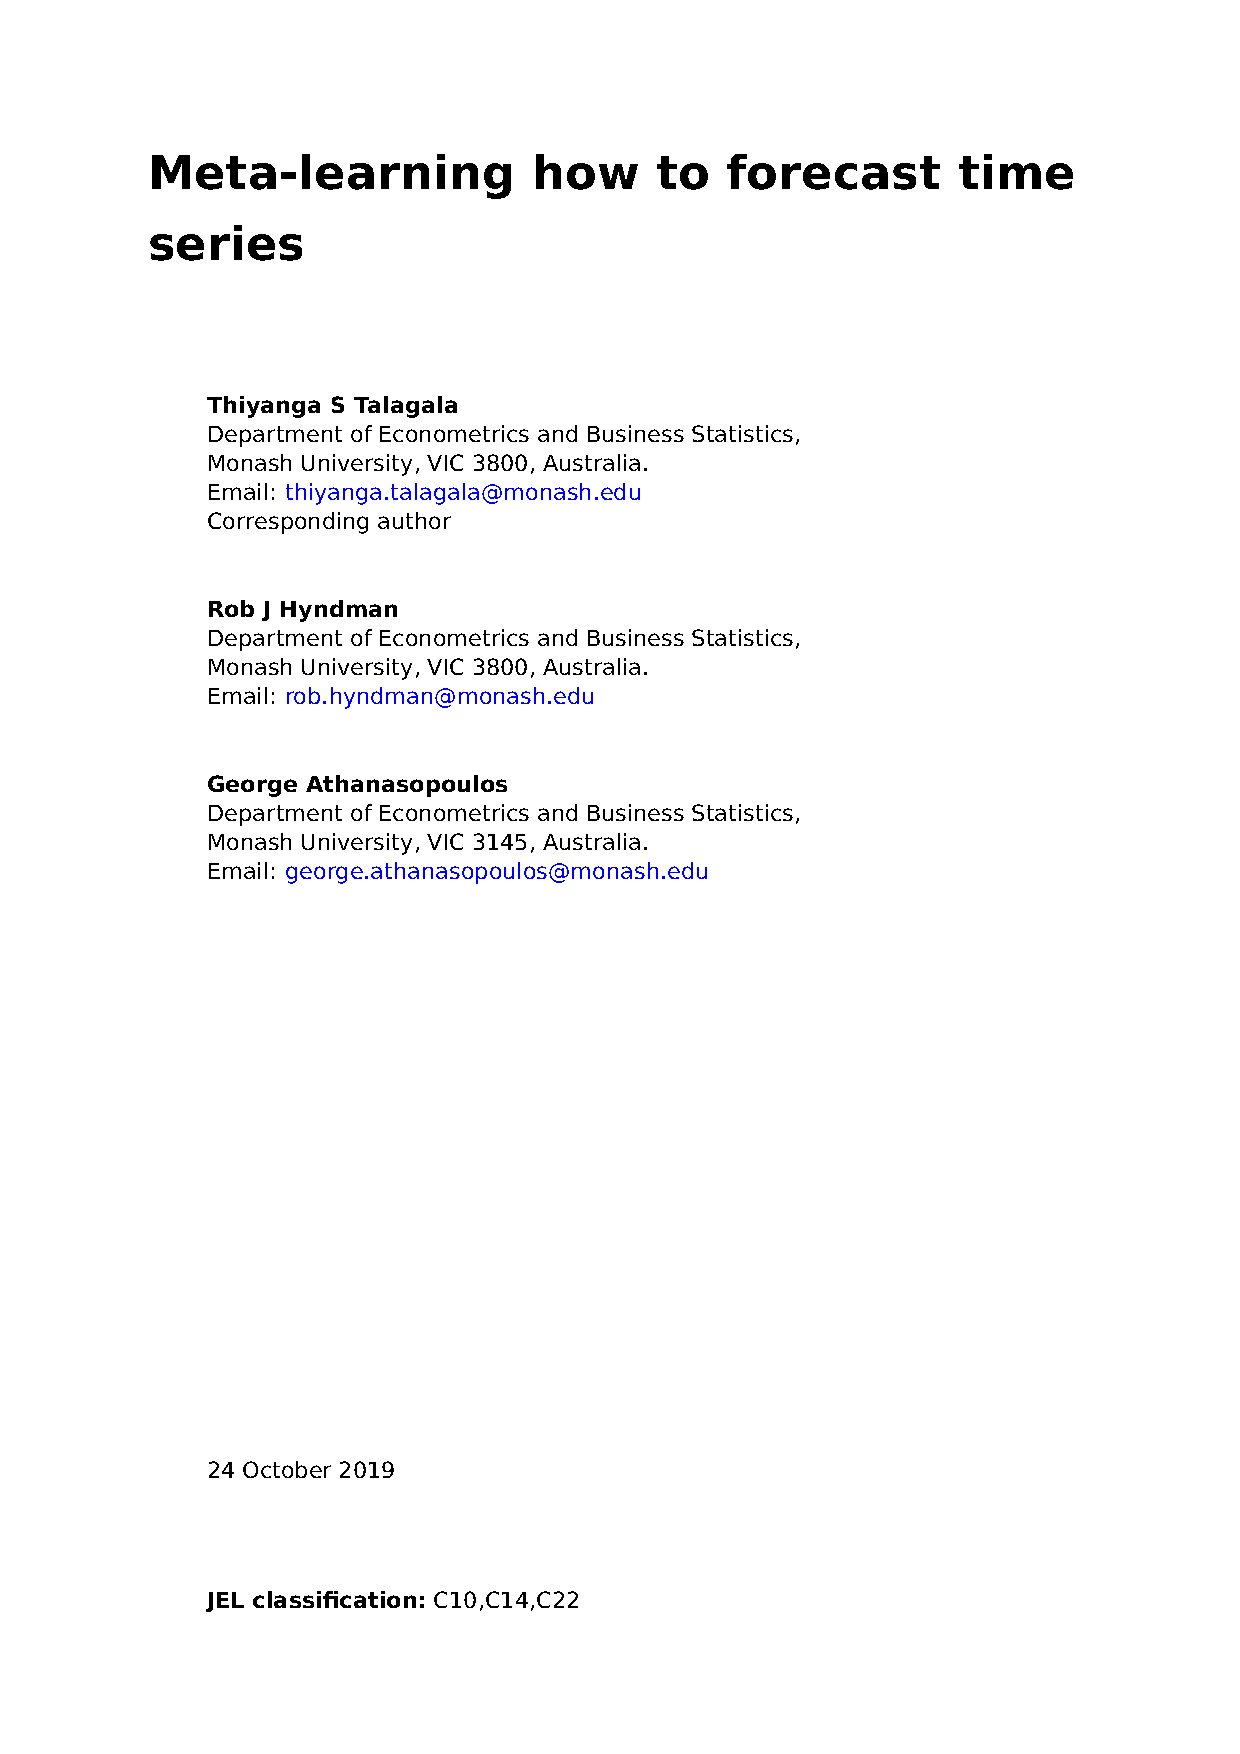
\includepdf[pages={1-31}, scale=1]{WorkingPaper1.pdf}

\hypertarget{ch:paper3}{%
\chapter{Peeking inside FFORMS: Feature-based forecast model selection}\label{ch:paper3}}

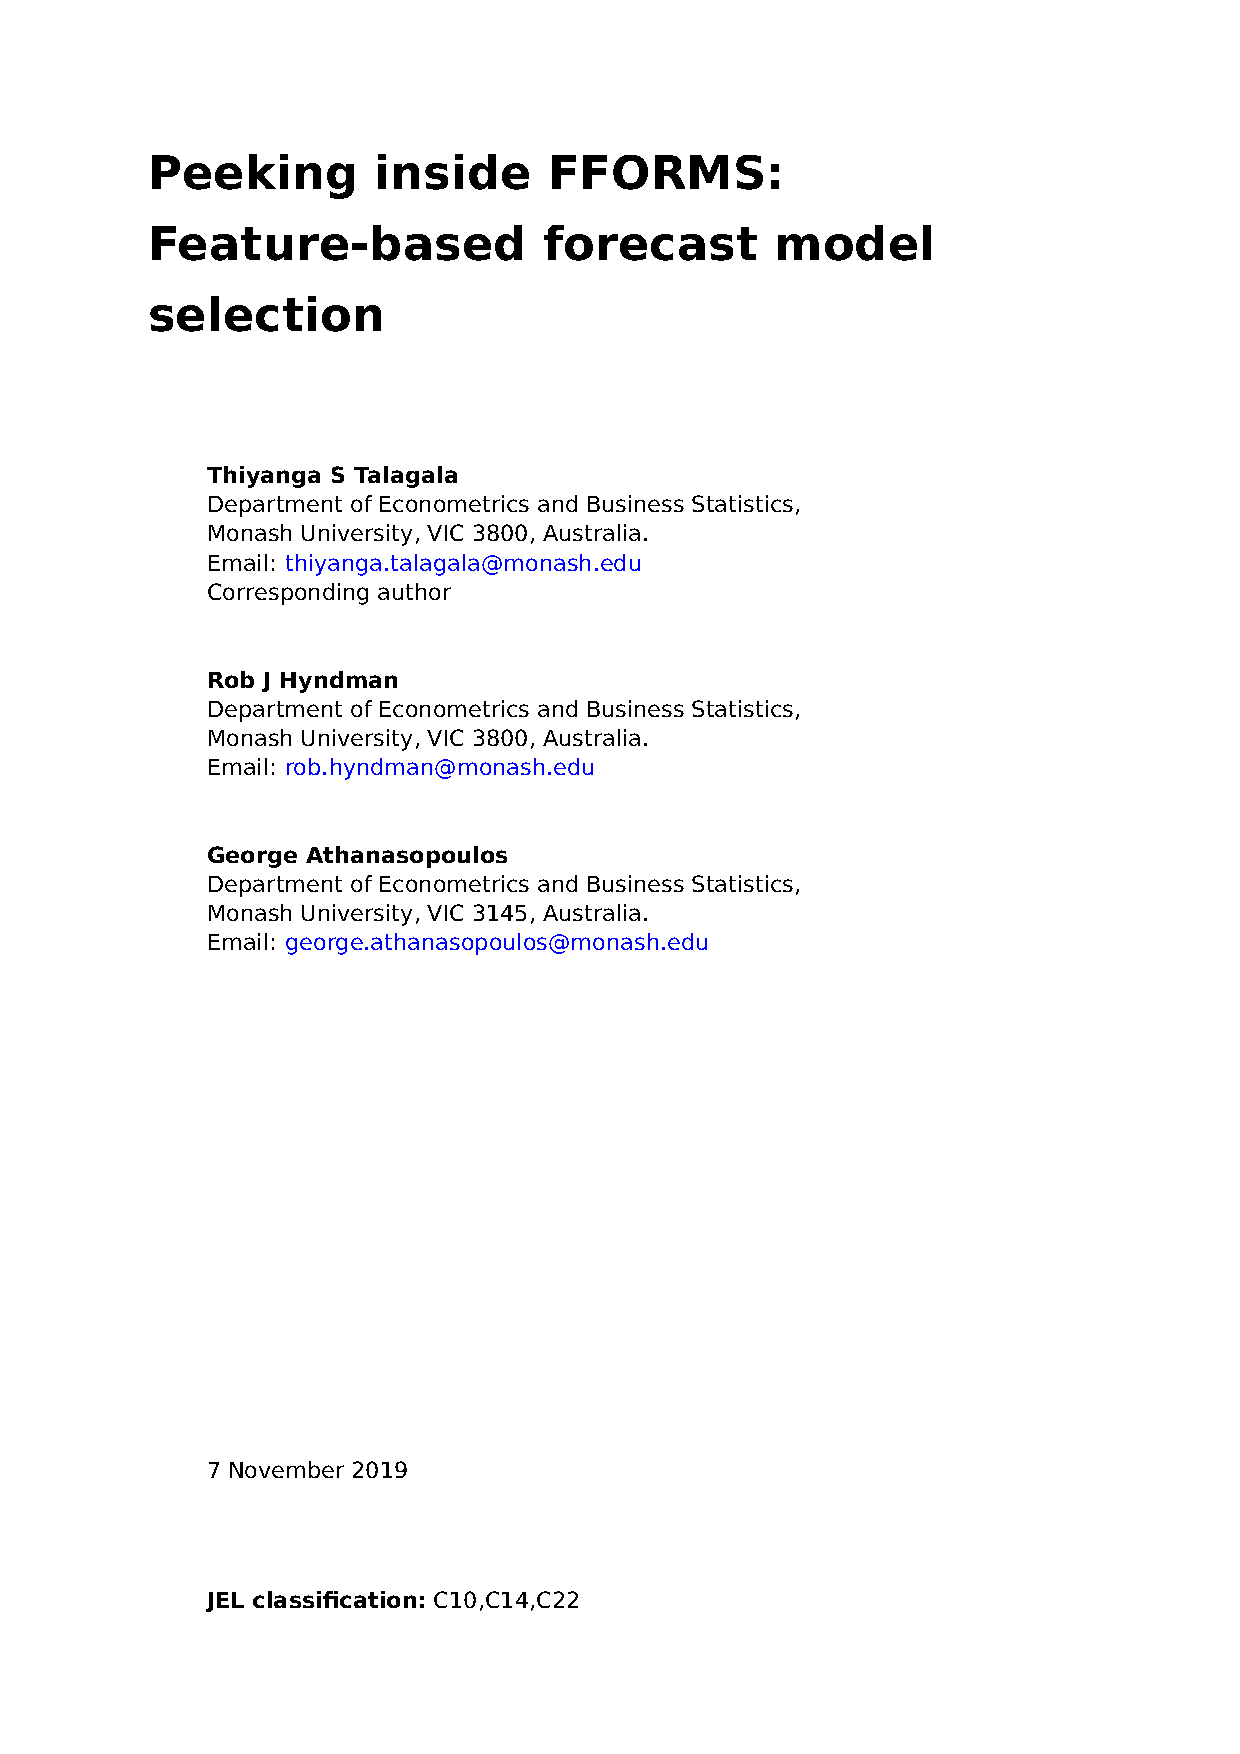
\includepdf[pages={1-45}, scale=1]{WorkingPaper2.pdf}

\hypertarget{ch:paper4}{%
\chapter{FFORMA: Feature-based forecast model averaging}\label{ch:paper4}}

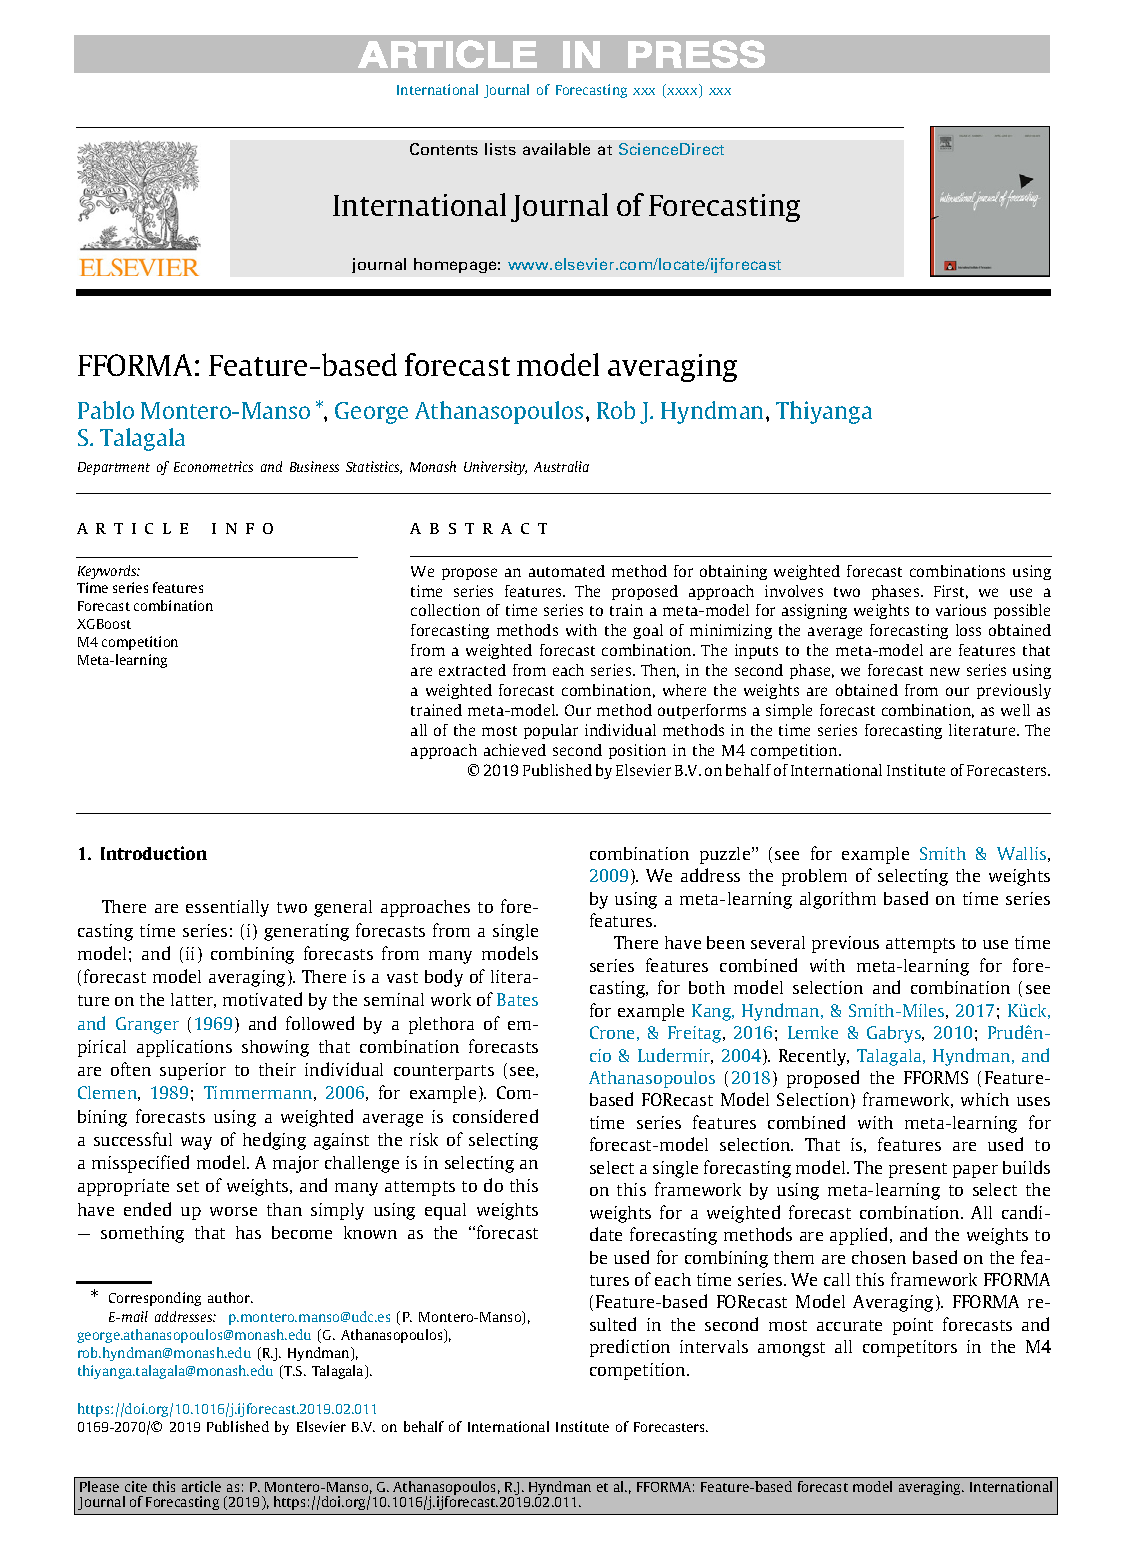
\includepdf[pages={1-7}, scale=1]{WorkingPaper3.pdf}

\hypertarget{ch:paper5}{%
\chapter{FFORMPP: Feature-based forecast model performance prediction}\label{ch:paper5}}

\includepdf[pages={1-29}, scale=1]{WorkingPaper4.pdf}

\hypertarget{ch:paper6}{%
\chapter{Conclusion}\label{ch:paper6}}

\hypertarget{summary-of-the-main-ideas-and-contributions}{%
\section{Summary of the main ideas and contributions}\label{summary-of-the-main-ideas-and-contributions}}

Forecasting is a key activity for any business to operate efficiently. Rapid advances in computing technologies have led to organisations being able to collect and access unimaginable amounts of time series data. Hence, many businesses require reliable and efficient ways for forecasting a large number of time series completely automatically. This thesis has presented three forecasting algorithms for large-scale applications. A fundamental aspect of the algorithms is the use of a meta-learning approach to guide a search for forecast model selection. In each of these algorithms, a vector of features calculated on time series becomes the input to the meta-learner. All the algorithms comprise two phases: the offline phase and the online phase. A key advantage of the algorithms is the idea of outsourcing most of the heavy computational work to the offline phase.

The work of this thesis covers four topics: i) time series features, ii) meta-learning, iii) machine learning interpretability and iv) automatic approaches for large-scale time series forecasting.

The main contribution of Chapter \ref{ch:paper2}, was to propose a meta-learning framework to identify the `best' forecast-model for each individual series. This framework is referred to as FFORMS: Feature-based FORecast-Model Selection. First a set of features that are useful in identifying suitable forecast models was identified, then extended by adding previously neglected features of time series.
The FFORMS framework builds a mapping that relates the features of a time series to the `best' forecast-model using a random forest. A key advantage of the proposed framework is that the time-consuming process of training a random forest is performed in the offline phase. The online phase involves calculating the features of a time series and using the pre-trained random forest to identify the best forecast model. Hence, generating forecasts only involves the estimation of a single model and computed forecasts based on the estimated model. In doing so, the FFORMS framework fills an important gap in contemporary forecasting practice, with many available models to choose from and with predictions being required extremely fast.

In Chapter \ref{ch:paper3}, the FFORMS framework was extended to handle weekly, daily and hourly series, as was the diversity of models used as class labels. The application of the FFORMS framework to the M4 competition data was analysed. The FFORMS approach yields accurate forecasts comparable to several benchmarks and other commonly used automated approaches for forecasting. The main contribution of Chapter \ref{ch:paper3} was the exploration of what is happening under the hood of the FFORMS framework, thereby presenting an understanding of what features lead to the different choice of models for forecasting and how different features influence the predicted outcome. This was accomplished using model-agnostic machine learning approaches. The chapter explored \textbf{which} features are the most important for the choice of the FFORMS framework, and \textbf{where} they are most important: that is, for the overall classification process, or within a specific class of models or a set of multiple classes of models. Further, partial dependency plots were used to visualise \textbf{when} and \textbf{how} these features link with the prediction outcome of the FFORMS framework. Finally, the chapter explored \textbf{when} and \textbf{how strongly} features interact with other features. For all features, the displayed relationships of partial dependency plots are consistent with the domain knowledge expectations. This is an important aspect in encouraging people to trust and use the proposed framework effectively.

In Chapter \ref{ch:paper4}, the main contribution was the new meta-learning framework FFORMA (Feature-based FORecast Model Averaging), which allows weights for forecast combinations to be obtained. An extreme boost gradient algorithm with a custom objective function was used to train a meta-model. Similar to FFORMS, the online part of the algorithm requires calculating the features of a time series and using the pre-trained XGBoost-based meta-learner. In FFORMA, the probabilities of each model being the best are used as weights for computing a combination forecast. FFORMA is slower than FFORMS because the final forecasts of FFORMA is the weighted average of several individual models. The FFORMA approach achieved second position in the M4 competition \autocite{makridakis2018m4}.

Chapter \ref{ch:paper5}, contributed the use of the efficient Bayesian multivariate surface regression approach to model forecast error as a function of features calculated from the time series. This is termed FFORMPP (Feature-based FORecast Model Performance Prediction). This framework took the correlation structure between forecast errors of different models into the meta-learner training process. FFORMPP allows ranking of the models with respect to their forecast errors and evaluates their relative forecast performance without calculating forecasts from all available individual models in the pool. The rankings of models provide an alternative solution to practitioners who may wish to incorporate their own judgements or expertise into the forecasting process.

One of the special components of the proposed meta-learning frameworks is augmenting the observed sample with simulated time series. This process may be useful when the number of observed time series is too small to build a reliable meta-learner. Alternatively, one might wish to add more of some particular types of time series to the reference set to achieve a more balanced sample. Chapter \ref{ch:paper2} and Chapter \ref{ch:paper3} explored a use of the model-based approach to simulate time series. The time series were simulated based on ARIMA and ETS models. The second contribution of Chapter \ref{ch:paper5} was to examine the feasibility of using a feature-based time series simulation approach in generating a realistic time series collection to obtain a diverse collection of time series. The chapter explored the use of GRATIS (GeneRAting TIme Series) with diverse and controllable characteristics proposed by \textcite{kang2019gratis}.

The third contribution of Chapter \ref{ch:paper5} was the exploration of the instance space defined by features to understand how certain features of the time series influence the forecast model selection. Previous work by \textcite{kang2017visualising} shows no dense concentration of instances according to the best forecast model of time series; the locations for which models are the best are scattered throughout the instance space. However, according to the results of Chapter \ref{ch:paper5}, dense regions are visible depending on which model is selected as a components of the calculation of combination forecasts. This also indicates that time series are not amenable to a single best forecast model but to a particular set of individual models. This visualisation of instances also follows \textcite{wickham2015visualizing}`s philosophy of 'representation of model in the data space (m-in-ds)'. Displaying the data in the model space (d-in-ms) is the most commonly used approach for model diagnostics, for example, a plot of fitted values versus residuals \autocite{wickham2015visualizing}. m-in-ds is a visualisation of embedding high-dimensional data into a low-dimensional space generated from the model. Visualisation of m-in-ds helps to gain an understanding of the nature of the relationship between features and predicted outcomes. In the context of classification, representation of m-in-ds could be achieved by first, projecting the training data set into meaningful low-dimensional feature space and second visualising the complete prediction regions or their boundaries. In other words, this can be considered the visualisation of predictor space in the context of data space.

A comparison of point forecasts values based on the three frameworks over the M4 competition data is shown in \autoref{forecastsconcl}. For each method, out-of-sample MASE over the forecast horizons was calculated and averaged over all time series. In general, FFORMA, and FFORMPP consistently forecast more accurately than all benchmark methods, except the random walk in daily series. FFORMA and FFORMPP performed equally well for yearly, quarterly and monthly series. For weekly, daily and hourly series, FFORMA provided substantially more accurate forecasts. The FFORMS approach also achieved comparable results in a much more cost- and time-effective manner. It is important to note that FFORMS forecasts are computed based on a single forecasting model (applying individual best forecast model to each series), FFORMA forecasts are computed based on a combination of nine different models and FFORMPP forecasts are computed by taking the median of individual forecasts corresponding to the four models with minimum predicted MASE. Hence, if the focus is to achieve reasonably accurate forecasts in a limited timeline, the FFORMS approach provides a solution. FFORMA is suitable if the aim is to achieve more accurate forecasts and the time and computing budget is not restricted. If the aim is to obtain reasonably accurate forecast using a reasonable time and computing budget, FFORMPP offers a promising solution for yearly, quarterly and monthly series. \textcolor{black}{The M4 competition winning method, hybrid Exponential Smoothing-Recurrent Neural Network (ES-RNN) approach is a synthesis of exponential smoothing model with advanced Long Short Term Memory (LSTM) neural networks} \autocite{smyl2019hybrid}\textcolor{black}{. The power of Slawek's ES-RNN approach lies in the co-training of both the per-time series exponential smoothing model parameters and the general RNN parameters in the deep learning layer of the architecture. According to} \autoref{forecastsconcl} \textcolor{black}{FFORMS approach outperformed ES-RNN approach for weekly series and FFORMA outperformed the ES-RNN for both weekly and daily series.} \textcolor{black}{Furthermore, a total of six  machine learning-based forecasting algorithms (5 submissions, 1 benchmark method based on MLP: multilayer perceptron) were considered in the M4 competition. These algorithms include simple neural network architectures as well as deep learning neural network architectures. All of them were less accurate than FFORMA and 5 of them were less accurate than FFORMS approach} \autocite{makridakis2019m4} \textcolor{black}{. Furthermore, these machine learning and deep learning forecast models can be easily integrated as part of the algorithm space in FFORMS, FFORMA and FFORMPP.}

\begin{table}[!h]
\centering\scriptsize\tabcolsep=0.12cm
\caption{MASE values calculated over the M4 competition data}
\label{forecastsconcl}
\begin{tabular}{l|rrrrrr}
\hline
\multicolumn{7}{c}{Point Forecasts (Mean Absolute Scaled Error (MASE))} \\\hline
 & Yearly & Quarterly & Monthly & Weekly & Daily & Hourly \\\hline
FFORMS & 3.17 &  1.20 &  0.98&  2.31& 3.57 &  0.84\\
FFORMA & 3.06 & 1.11 &  0.89& 2.11 & 3.34 & 0.81\\
FFORMPP & 3.07 & 1.13 &  0.89& 2.46 & 3.62 & 0.96\\\hline
auto.arima & 3.40 &1.17  &0.93  & 2.55 &  -& - \\
ets & 3.44 &  1.16& 0.95 &  -&-  &  -\\
theta & 3.37 &1.24  & 0.97 &2.64  & 3.33 & 1.59 \\
rwd & 3.07 & 1.33 & 1.18  & 2.68  & 3.25 & 11.45 \\
rw & 3.97 & 1.48 & 1.21  &2.78  & 3.27 & 11.60 \\
nn & 4.06 & 1.55 &  1.14 &4.04 & 3.90 & 1.09 \\
stlar & - & 2.02 &  1.33& 3.15 & 4.49 & 1.49 \\
snaive & - &  1.66& 1.26 &  2.78& 24.46 & 2.86 \\
tbats & - & 1.19 &  1.05& 2.49 & 3.27 &  1.30\\
wn & 13.42 &  6.50&  4.11&  49.91& 38.07 & 11.68 \\
mstlarima & - & - &  - & - & 3.84 &  1.12\\
mstlets & - &  - &  - &  - & 3.73 &  1.23\\
combination (mean) & 4.09 & 1.58 &  1.16&6.96  & 7.94 & 3.93 \\\hline
M4-1st & 2.98 & 1.12 &  0.88& 2.36 & 3.45 & 0.89\\\hline
\end{tabular}
\end{table}

\begin{table}[!h]
\centering\scriptsize\tabcolsep=0.12cm
\caption{Computational time for producing forecasts based on 100 randomly selected series from each frequency category of the M4 data set.}
\label{forecasttime}
{\color{black}\begin{tabular}{l|rrrrrr}
\hline
\multicolumn{7}{c}{Computational time for producing forecasts in seconds (IQR)} \\\hline
 & Yearly & Quarterly & Monthly & Weekly & Daily & Hourly \\\hline
FFORMS & 3.38 (0.18) & 20.98 (8.23)  &  100.13 (7.13) & 128.41 (5.17)  & 77.20 (5.67) & 34.53 (5.16) \\
FFORMA & 23.41(0.26) & 144.39 (0.60)& 873.25 (0.32) & 718.68 (5.24) & 886.33 (6.31) & 821.98 (5.42) \\
FFORMPP & 5.31(0.21) & 30.45 (1.44) & 190.05 (5.15) & 183.36 (6.78) & 93.76 (0.34) & 56.14 (11.67) \\\hline
auto.arima & 5.91 (0.05)  &  42.11 (2.15)& 448.41 (1.95) & 584.98 (2.35) &  -& - \\
ets & 1.14 (0.02) & 16.92 (0.09) & 115.50 (0.17) &  -&-  &  -\\
theta & 2.74 (2.48) & 10.15 (11.45) & 29.13 (1.15) & 96.06 (0.42) & 83.77 (2.67) & 54.32 (2.32) \\
rwd & 0.29 (5.42) & 0.29 (8.20) & 0.33 (15.57)  & 0.34 (21.78)  & 0.41 (33.72)  & 0.37 (26.46) \\
rw & 0.16 (4.65) & 0.20 (6.67) & 0.26 (15.68)   & 0.22 (17.16) &0.27 (19.56)  & 0.24 (9.58)\\
nn & 2.32 (0.14) & 6.54 (0.23) & 32.78(0.25) &281.68 (0.61) & 424.28 (1.71) & 354.97 (3.61) \\
stlar & - & 0.83 (17.97) & 0.94 (12.03) & 0.90 (10.11) & 2.21 (0.12) & 1.70 (0.01) \\
snaive & - & 0.18 (4.51) & 0.30 (3.12) & 0.20 (1.44) & 0.32 (0.34) & 0.44 (2.12) \\
tbats & - & 20.16 (6.98) & 38.12 (2.44) & 40.16 (3.36) & 68.73 (0.65) & 49.52 (2.98) \\
wn & 0.19 (2.65) & 0.20 (4.30) & 0.23 (0.08) & 0.19 (4.51) & 0.26 (1.00) & 0. 22 (0.05) \\
mstlarima & - & - &  - & - & 86.92 (0.52) & 30.60 (0.17) \\
mstlets & - &  - &  - &  - & 19.79 (0.09) & 10.13 (0.48)\\\hline
\end{tabular}}
\end{table}

\begin{table}[!h]
\centering\scriptsize\tabcolsep=0.12cm
\caption{Computational time for features over 100 time series.}
\label{featuretime}
{\color{black}\begin{tabular}{lll|r}
\hline
\thead{Feature category \\ (as in "tsfeatures" \\ package)}        & \multicolumn{1}{l}{Feature} & Description &  \thead{Computational time \\ (median/(IQR))}                 \\ \hline
                 & \multicolumn{1}{l}{T} & length of time series &           47 (3) nanoseconds        \\ \hline
\multirow{12}{*}{stl\_features } &            trend           & strength of trend  & \multirow{12}{*}{862.45 (5.27) milliseconds} \\
                   &            seasonality           & strength of seasonality  &                    \\
                   &      linearity                 & linearity &                    \\
                   &          curvature             & curvature &                    \\
                   &          spikiness             & spikiness &                    \\
                   &      e\_acf1                 & first ACF value of remainder series &                    \\
      &           e\_acf10            & sum of first 10 ACF value of remainder series &                    \\
                   &      peak                 & strength of peak &                    \\
                   &     nperiods                  & number of seasonal periods in the series &                    \\
                   &          trough             & strength of trough &                    \\
                   &           seasonal\_period            & length of seasonal period &                    \\\hline
    hurst               & \multicolumn{1}{l}{hurst } & Hurst exponent  &    83.31 (4.79) milliseconds               \\ 
      stability             & \multicolumn{1}{l}{stability} & stability &      80.24 (4.16) milliseconds             \\ 
      lumpiness             & \multicolumn{1}{l}{lumpiness} & lumpiness &    154.22 (2.08) milliseconds               \\ 
      entropy             & \multicolumn{1}{l}{entropy} & spectral entropy &    247.57 (5.31) milliseconds              \\ 
     nonlinearity              & \multicolumn{1}{l}{nonlinearity} & nonlinearity &  255.57 (2.53) milliseconds                 \\ \hline
\multirow{2}{*}{holt\_parameters}  & \multicolumn{1}{l}{alpha} & ETS(A,A,N) $\hat\alpha$ & \multirow{2}{*}{367.50 (6.84) milliseconds}  \\ 
                   & \multicolumn{1}{l}{beta} & ETS(A,A,N) $\hat\beta$   &                    \\ \hline
\multirow{3}{*}{hw\_parameters}  & \multicolumn{1}{l}{hwalpha} & ETS(A,A,A) $\hat\alpha$   & \multirow{3}{*}{4.89 (0.08) seconds}  \\ 
                   & \multicolumn{1}{l}{hwbeta} & ETS(A,A,A) $\hat\beta$  &                    \\
                   & \multicolumn{1}{l}{hwgamma} & ETS(A,A,A) $\hat\gamma$  &                    \\ \hline
    unitroot\_pp               & \multicolumn{1}{l}{ur\_pp} & test statistic based on Phillips-Perron test  &           174.44 (1.66) milliseconds      \\ 
 unitroot\_kpss                  & \multicolumn{1}{l}{ur\_kpss} & ur\_kpss &  66.44 (4.25) milliseconds                  \\ \hline
\multirow{7}{*}{acf\_features}  & \multicolumn{1}{l}{y\_acf1} & first ACF value of the original series   & \multirow{7}{*}{255.23 (3.85) milliseconds }  \\
                   & \multicolumn{1}{l}{y\_acf10 } & sum of squares of first 10 ACF values of original series  &                    \\ 
                   & \multicolumn{1}{l}{diff1y\_acf1} & first ACF value of the differenced series  &                    \\ 
                   & \multicolumn{1}{l}{diff1y\_acf10 } &sum of squares of first 10 ACF values of differenced series   &                    \\ 
                   & \multicolumn{1}{l}{diff2y\_acf1} & first ACF value of the twice-differenced series &                    \\ 
                   & \multicolumn{1}{l}{diff2y\_acf10} & sum of squares of first 10 ACF values of &                    \\ 
                   & \multicolumn{1}{l}{seas\_acf1} & autocorrelation coefficient at first seasonal lag &                    \\ \hline
            & \multicolumn{1}{l}{ lmres\_acf1} & first ACF value of residual series of linear trend model  &        50.21 (2.34) milliseconds            \\ \hline
\multirow{5}{*}{pacf\_features}  & \multicolumn{1}{l}{y\_pacf5} & sum of squares of first 5 PACF values of original series & \multirow{5}{*}{313.39 (5.73) milliseconds }  \\ 
                   & \multicolumn{1}{l}{diff1y\_pacf5} & sum of squares of first 5 PACF values of differenced series &                    \\ 
                   & \multicolumn{1}{l}{diff2y\_pacf5} & sum of squares of first 5 PACF values of twice-differenced series  &                    \\ 
                   & \multicolumn{1}{l}{seas\_pacf} & partial autocorrelation coefficient at first seasonal lag  &                    \\  \hline
crossing\_points                   & \multicolumn{1}{l}{crossing\_points} & number of times the time series crosses the median &   26.73 (2.62) milliseconds                \\
  arch\_stat                 & \multicolumn{1}{l}{ARCH.LM} & ARCH LM statistic & 135.47 (3.26) milliseconds                  \\ \hline
   heterogeneity                & \multicolumn{1}{l}{arch\_acf} & sum of squares of the first 12 autocorrelations of $z^2$ &     441.63 (6.04) milliseconds              \\ 
\multirow{4}{*}{}  & \multicolumn{1}{l}{garch\_acf} & sum of squares of the first 12 autocorrelations of $r^2$ & \multirow{4}{*}{}  \\ 
                   & \multicolumn{1}{l}{arch\_r2} & $R^2$
                   value of an AR model applied to $z^2$ &                    \\ 
                   & \multicolumn{1}{l}{garch\_r2} & $R^2$
                   value of an AR model applied to $r^2$ &                    \\ \hline
\end{tabular}}
\end{table}

One limitation of the analysis is that it does not report the computational time owing to different platforms used to run the frameworks. However, all three frameworks are scalable both in time and computing costs. Further, all three frameworks can be easily parallelised for a given computing budget by dividing the process into separate steps. \textcolor{black}{To ensure a fair comparison, computational time for producing forecasts based on 100 randomly selected series from each frequency category of the M4 competition data set is given in} \autoref{forecasttime}\textcolor{black}{. The reported values are median elapsed time of 100 replicates. The corresponding Inter Quartile Ranges (IQRs) are given in parentheses.} \autoref{featuretime} \textcolor{black}{reports the computational time for features. None of the features are computationally demanding.} \textcolor{black}{The computational time was measured using the R package microbenchmark} \autocite{microbenchmark} \textcolor{black}{on 24 core Xeon-E5-2680-v3 @ 2.50GHz servers.}

\textcolor{black}{According to Table 4 in Chapter} \ref{ch:paper2} \textcolor{black}{and Table 7 in Chapter} \ref{ch:paper5}\textcolor{black}{, the most accurate forecast models are the ones that most frequently get selected by the meta-learners. For example, according to} \autoref{forecastsconcl} \textcolor{black}{the random walk with drift performs extremely well with yearly series. According to Table 4 in Chapter} \ref{ch:paper2} \textcolor{black}{the random walk with drift has been selected 46.75\% of the time by FFORMS and according to Table 7 in Chapter} \ref{ch:paper5} \textcolor{black}{the random walk with drift has been selected as one of the components in calculating combination forecasts for all series by FFORMPP. The interpretations for other frequency categories can be made in a similar fashion. Further, across all frequency categories white noise process was the least selected forecast model and according to } \autoref{forecastsconcl} \textcolor{black}{it was the worst performing model across all frequency categories. Since, the white noise process turned out to be the least accurate, it was not considered as a base model to the algorithm space of FFORMA. This helped to reduce the computing time while maintaining its high accuracy. Hence, prior knowledge about the forecast accuracy of base models can be used to reduce the number of models to be used in the algorithm space. This will intern speed up the both online and offline phases of the classification  process without losing too much information.}

\textcolor{black}{In our algorithms we use a large sample of time series to create a reference set for training the meta-learners. Since the processing of data to create the reference set is done in the off-line phase of the algorithms, the computational time is of no real consequence.  However, it could be the case that the meta-learner should be re-trained once in a while. For example, that could happen in a retail company where the meta-learner is trained with its own data to forecasts the sales of its own products which features may significantly change over time. In order to get an idea about when and how often the re-training process should be done, two-dimensional instance space, defined by the features could be used. For that, we first compute the principal components projection using the features in the reference set, and then project the new time series to the same low-dimensional feature space. If the new time series fall within the space covered by the series in the reference set a new meta-learner is not required. If any of the series fall out-side of the space covered by the reference set a new-meta learner is required to be trained.}

\textcolor{black}{One could argue in the FFORMS algorithm, the random forest probability scores  could be used for weighting alternative forecast models and construct a robust combination scheme like FFORMA. However, this approach did not bring any improvement in the performance and furthermore with some series it degraded the performance. The reason is that in FFORMS the forecast model selection problem is treated as a classification problem. Hence, in this case the weights are mostly close to either 0 and 1; the best model has a weight close to 1 and others very close to 0. For example, suppose for a given series the forecast error vector for the random walk, the random walk with drift and a white noise process is [1.31, 1.30, 3.4]. Then, ideally the vector of class weight we expect from FFORMS is [0, 1, 0], i.e. the best model is given class probability 1 and others 0. This limitation motivated us to introduce FFORMA. In forecast-combinations we would expect similar weights for the random walk with drift and the random walk as they both perform equally well. For this, in the objective function of FFORMA, instead of minimizing the classification error we minimize the average forecast error to obtain suitable weights for forecast combinations.} \textcolor{black}{In FFORMPP we opt for simplicity. The median of the best four models is used to compute the combination forecasts. As} \textcite{lichtendahl2013better} \textcolor{black}{claim the simpler method
of averaging the quantiles, seems to give as good as a result as more elaborate ones. This helps to reduce the computational time while maintaining accuracy.}

\textcolor{black}{All our frameworks are robust to outliers present in the time series. Furthermore, with the exception of Spectral Entropy all other features are not affected by missing values. For the case of calculating Spectral Entropy snaive and naive approaches are used to impute missing values, before computing the feature. However, both the feature space and algorithm space will depend on the specific population of time series models we need to forecast. Hence, a limitation of these frameworks is that expert's knowledge is required to decide the models to be included in the algorithm space and the features to be included in the feature space.}

\hypertarget{software-development-and-research-reproducibility}{%
\section{Software development and research reproducibility}\label{software-development-and-research-reproducibility}}

\hypertarget{software}{%
\subsection{Software}\label{software}}

Two R packages were developed based on the frameworks introduced in this thesis.

\begin{enumerate}
\def\labelenumi{\arabic{enumi}.}
\item
  The first R package \texttt{seer} is an accompaniment to the framework proposed in Chapter \ref{ch:paper2}.
  The package is available at \url{https://github.com/thiyangt/seer}. To the best of my knowledge \texttt{seer} is the first R package to implement the meta-learning framework for time series forecasting.
\item
  The second R package, \texttt{fformpp}, is an accompaniment to the framework proposed in Chapter \ref{ch:paper5}. The package is available at \url{https://github.com/thiyangt/fformpp}.
\end{enumerate}

\hypertarget{reproducibility}{%
\subsection{Reproducibility}\label{reproducibility}}

\textcite{peng2015reproducibility} writes,

\begin{quote}
``Reproducibility is defined as the ability to recompute data analytic results, given an observed
data set and knowledge of the data analysis pipeline. Replicability and reproducibility are two
foundational characteristics of a successful scientific research enterprise.''
\end{quote}

Research reproducibility is an important component for research sustainability. The R codes to reproduce all results and figures of each paper are available in the following Github repositories.

Chapter \ref{ch:paper2}: \url{https://github.com/thiyangt/WorkingPaper1}

Chapter \ref{ch:paper3}: \url{https://github.com/thiyangt/FFORMSinterpretation}. Further, the R package \texttt{explainer} contains the main functionalities used to generate partial dependence plots is available at \url{https://github.com/thiyangt/explainer}

Chapter \ref{ch:paper4}: \url{https://github.com/robjhyndman/fforma-paper}

Chapter \ref{ch:paper5}: \url{https://github.com/thiyangt/chapter5_fformpp}

The R codes to reproduce the content of this PhD this are available at \url{https://github.com/thiyangt/PhDThesis}

For all papers, \texttt{Rmarkdown} was used to produce a readable output file, supported by the \texttt{rmarkdown}, \texttt{knitr} and \texttt{pander} packages. The R package \texttt{bookdown} was used to produce a readable output file of this PhD thesis with the support of the Monash University PhD thesis template available at \url{https://github.com/robjhyndman/MonashThesis}.

\hypertarget{future-directions}{%
\section{Future directions}\label{future-directions}}

The results clearly demonstrate that features of time series are useful in identifying suitable models for forecasting. There are several directions for future research.

\begin{enumerate}
\def\labelenumi{\arabic{enumi}.}
\item
  \emph{Application to other datasets.} \textcolor{black}{The current applications are limited to M1, M3 and M4 competition datasets. Therefore, the applicability of the proposed frameworks is limited to groups of time series of similar attributes as the data in the M-competitions. For example, the proposed frameworks with the same set of features and forecast models might not be the right choice for forecasting stock return data, or irregular time series, etc. Hence, it is important to expand the frameworks to other datasets that come from different application domains. When adapting the frameworks to other applications the feature space should be revised with appropriate features that measure characteristics of interest. The algorithm space should also be revised with suitable forecast models. A suitable forecast error metric should also be considered to evaluate the performance of different forecast models. For example, retail companies collect a large number of time series related to sales data. Most of these series are intermittent in nature} \autocite{seaman2018considerations}. \textcolor{black}{Low-volume and intermittent time series were not considered in the M-competition} \autocite{makridakis2019m4}. \textcolor{black}{Hence, new features such as proportion of zeros, number of non-zero intervals, kurtosis, etc., need to be selected to the feature space. The use of forecast error metrics such as sMAPE with intermittent series is not also suitable as it would involve division by zero. Furthermore, none of the time series in the M-competition collections have negative values. Hence, these are not representative of stock return series. New features need to be included when adapting the frameworks for such situations. In addition to the new features new forecast model such as ARCH, GARCH, etc. also need to be considered for the algorithm space.}

  \textcite{smith2015generating} \textcolor{black}{pointed out the importance of evaluating meta-frameworks using simulated time series with different distributions in the feature space to achieve a better understanding of strengths and weaknesses of algorithms. Hence, in addition to the application of these frameworks to real-world data sets, the GRATIS} \autocite{kang2019gratis} \textcolor{black}{approach can be used to create a test bed with controllable features of the instances to evaluate the frameworks. An illustrative example of the idea is shown in Figure} \ref{fig:example}\textcolor{black}{. First the features of yearly M3 series are computed. Principal component analysis is used to project these onto a two-dimensional space referred to as "instance space".  The green points correspond to the yearly time series from the M3 competition. The orange points are the target points. The rules learned by a meta-learner trained based on the green points do not claim to be universally applicable, they merely hold for time series with similar feature distribution as M3 data. Hence, to make the meta-learner more generalizable a more diverse collection of time series can be considered that fills and spreads out the instance space. The GRATIS approach can be used to   generate new time series from the target points. Note that it is not possible to generate time series from some target points due to natural constraints in feature combinations} \autocite{kang2017visualising}\textcolor{black}{. According to the no free lunch theorem, there is no algorithm that performs best for all kinds of problems. Hence, the application of the frameworks to simulated time series with controllable features will help the understanding of when these frameworks perform well and when they fail. This will provide a valuable insight to improve the generalisability of the frameworks.}
\end{enumerate}

\begin{figure}
\centering
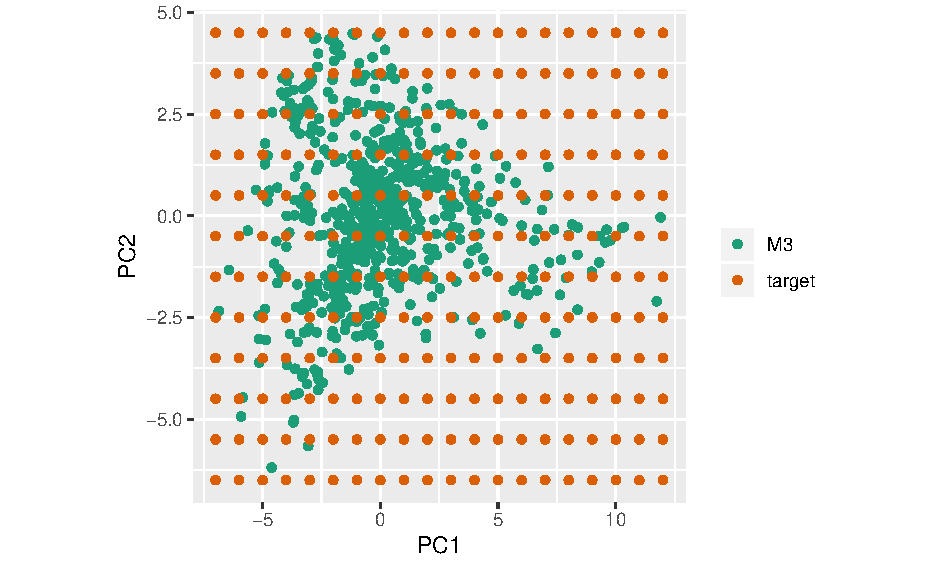
\includegraphics{thesis_files/figure-latex/example-1.pdf}
\caption{\label{fig:example}Instance space of yearly M3 time series. PC1 and PC2 are the first two principal components, projected from the features of the yearly M3 time series. The green points are the yearly M3 time series and the orange points are the target points.}
\end{figure}

\newpage

\begin{enumerate}
\def\labelenumi{\arabic{enumi}.}
\setcounter{enumi}{1}
\item
  \emph{Feature set.} Another important direction for future work is to investigate spectral-domain time series features such as wavelet transform-based features of the time series and spectral density-based features. \textcolor{black}{For example, number of peaks in the global wavelet power spectrum, standard deviation of the wavelet coefficients, etc. It is important to test whether these features would lead to better results for any of the algorithms.}
\item
  \textcolor{black}{\textit{Feature engineering for meta-learning.} The choice of time series features used in the thesis was rather adhoc in nature and developed mostly based on intuition.} \textcolor{black}{In Chapter} \ref{ch:paper3}\textcolor{black}{, a throughout empirical exploration of features was performed to understand how different features and their interactions affect the choice of forecast model.  Identification of a good feature subset is an important component in the meta-learning process, as all our algorithms depend crucially on finding features that enable identification of the best forecast model for the given time series.  A good set of features will not only speed up the calculation process, they will help to obtain even better results. Hence, further research is needed to answer the following contrasting challenges confronting us when designing a meta-learning framework.}

  \textcolor{black}{3.1: Do we need to add more features? The frameworks introduced in the thesis considered a pool of more than 30 features. However, are these enough? How much information is lost by considering only these features? Is there any possible way to measure the complete information provided by a time series and therefore, to measure the information we miss by using a subset of features to capture it?}

  \textcolor{black}{ 3.2: Do we need all the features used in the frameworks? Would it be possible to achieve similar accuracy level by selecting a subset of features?}

  \textcolor{black}{At the same time, the number of features considered will influence the choice of algorithm used for training. For example, if a single decision tree is considered, then the use of 30 features is probably ineffective as the algorithm is too simplistic to model the connection between forecast model performance and features.  However, the algorithms such as random forest, deep-learning architectures can effectively model such complex relationships. Hence, further research is needed to explore if feature engineering process would lead to better results for any of these algorithms in terms of accuracy as well as time.}
\item
  \textcolor{black}{\textit{Meta-learner training process.} An important component of a meta-learning framework is the construction of an engine that maps an input space composed of features to an output space composed of forecast model performance. Another direction to investigate could be to replace the training algorithm with other alternatives such as deep-learning architectures, support vector machines, etc. and test whether these approaches outperform the FFORMS, FFORMA and FFORMPP frameworks.}
\item
  \emph{Probabilistic forecasting.} \textcolor{black}{An interesting extension would be to apply this methodology for producing probabilistic forecasts rather than point forecasts. To account for this, instead of using MASE as the error measure in the offline phase, it could be replaced by a scale-free scoring rule such as log scores and retrain a meta-learner for probabilistic forecasting.}
\item
  \emph{Fast and furious forecasting.} Another strand of research would allow for clustering of time series, with a similar forecasting model being applied to all series within a cluster. \textcite{ashouri2019tree} \textcolor{black}{provides a brief survey of such methods.} In this way, the number of models to be estimated can be greatly reduced. However, the approach would lead to a loss of efficiency in using non-optimal parameters, and additional variance might be incurred from potentially selecting a non-optimal forecasting method for a given series. It is important to explore how to balance these effects against the speed improvements that are achieved.
\end{enumerate}

\printbibliography[heading=bibintoc]



\end{document}
